%%%%%%%%%%%%%%%%%%%%%%%%%%%%%%%%%%%%%%%%%%%%%%%%%%%%%%%%%%%%%%%%%%%%%%%%%%%%%%%%%%%%%%%%%%%%%%%%%%%%%%%
% Soutenance 2
% Bitume Legends Project
% CarrEniX
% Avril 2022
%%%%%%%%%%%%%%%%%%%%%%%%%%%%%%%%%%%%%%%%%%%%%%%%%%%%%%%%%%%%%%%%%%%%%%%%%%%%%%%%%%%%%%%%%%%%%%%%%%%%%%%

% Packages
\documentclass[12pt,a4paper]{article}
\usepackage{mathtools}
\usepackage[utf8]{inputenc}
\usepackage{graphicx}
\usepackage[french]{babel}
\usepackage[T1]{fontenc}
\usepackage{url}
\usepackage{fancyhdr}
\usepackage{longtable}
\usepackage[aboveskip=.5cm]{caption}
\usepackage{pdflscape}
\usepackage{geometry}
\usepackage{xcolor}

% Global settings of document
\setlength\parindent{20pt}
\newcommand{\btmlgs}{\textsl{Bitume Legends}}
\newcommand{\AI}{Intelligence Artificielle}
\newcommand{\FL}{\textsl{FL Studio 20}}
\newcommand{\CEX}{\textsc{CarrEniX}}
\newcommand{\SITE}{\(\mathtt{btms.games}\)}
\newcommand\ytl[2]{\parbox[b]{10em}{\hfill{\color{cyan}\bfseries\sffamily 
    #1}~$\cdots\cdots$~}\makebox[0pt][c]{$\bullet$}\vrule\quad 
    \parbox[c]{5cm}{\vspace{7pt}\color{red!40!black!80}\raggedright\sffamily #2\\[7pt]}\\[-3pt]}
\pagestyle{fancy}
\rhead{\btmlgs}
\lhead{Rapport de Soutenance Intermédiaire}
\rfoot{Page \thepage}
\lfoot{\CEX}
\fancyfoot[C]{}
\setlength{\headheight}{15pt}
\geometry{textheight=600pt}
\renewcommand{\listfigurename}{Table des Annexes}
\renewcommand{\contentsname}{Table des Matières}
\graphicspath{{../Medias}}

% Begin of the document
\begin{document}

    \begin{titlepage}
        \newcommand{\HRule}{\rule{\linewidth}{0.5mm}}
        \center
        \text{\LARGE Projet \btmlgs}\\[1cm]
        
\includegraphics[scale=0.7]{logo192.png} \\[1cm]
        \HRule \\[0.4cm]
        { \huge \bfseries Rapport de Soutenance Intermédiaire\\[0.3cm] }
        \HRule \\[1.5cm]
        {\large \bfseries \CEX} \\[0.3cm]
        Anthony \textsc{Caron}\;--\;Melvyn \textsc{Delaroque}\\
        Victorien \textsc{Cambourian}\;--\;Xavier \textsc{de Place}
        \\ [4.5cm]
        EPITA INFOSUP 2026\\Année 2021 - 2022\\
        \SITE
    \end{titlepage}

    \tableofcontents
    \clearpage

    \addcontentsline{toc}{section}{Introduction}
    \section*{Introduction}
        Nous sommes le studio \CEX\, qui développe \btmlgs, un jeu de course automobile 3D en
        \textit{low-poly}. Après avoir commencé le projet début janvier, et présenté notre avancée 
        mi-mars, nous publions notre second rapport. Il permet de faire le point sur ce que nous avons
        fait, les objectifs atteints, les priorités ainsi que les ressources utilisées durant ce 
        projet.\\
        Dans ce second rapport, nous allons aborder l'avancée de notre projet, les modifications que 
        nous avons du apporter suite à la première soutenance, les problèmes et difficultés auxquels 
        nous nous sommes confrontés, comment nous les avons les régler, le ressenti des membres durant 
        cette deuxième période ainsi que nos objectifs pour la troisième et dernière soutenance.

    \section{Avancées}
        Pour récapituler les avancées du projet, nous avons repris point par point les objectifs de 
        notre rapport de première soutenance et nous avons comparé notre point d'avancement et nos 
        prédictions. Et le résultat est concluant:

        \subsection{Graphisme}
            Au lancement du projet, nous voulions créer nous même nos voitures et nos circuit à 
            l'aide du logiciel de modélisation 3D Blender. Toutefois, cela prends beaucoup de temps,
            temps qui n'est pas utilisé à coder le jeu, résoudre des bugs, etc. Nous avons donc fait
            un compromis entre notre volonté de créer nous même le design du jeu et la contrainte de
            temps. Nous nous sommes orientés alors sur l'ajout d'un \textit{asset} du \textsl{Unity
            Asset Store}, pour obtenir des voitures et des morceaux de pistes. Ceci nous a permis de
            créer directement dans \textsl{Unity} nos différents circuits et de gagner beaucoup de 
            temps. 
        
        \subsection{Sauvegarde}
            Pour que notre jeu soit plus facile à appréhender, nous avons créé un système de 
            sauvegarde. Il est composé de 2 principe : le \textsl{Save}, qui permet d'enregistrer 
            les données voulues et nécessaires au bon fonctionnement du jeu, ainsi que le 
            \textsl{Load}, qui permet de charger la sauvegarde lors du lancement du jeu. Pour le 
            moment, il s'occupe uniquement de sauvegarder quelle voiture a été choisie dans le 
            garage et de l'enregistrer pour la charger lors du prochain lancement du jeu. À terme, 
            nous comptons sauvegarder l'expérience du joueur, son pseudo, ainsi que la possible 
            customisation de ses voitures.

        \subsection{Menu}
            Pour la première soutenance, nous avons fait une charte graphique et un design pour les 
            menus.
            Nous nous étions concentrés sur le menu principal. Pour cette seconde soutenance, nous 
            avons travaillé les
            sous-menus des différents modes de jeu et les fonctionnalités internes.\\
            Nous avons implémenté le garage, permettant de
            sélectionner une voiture pour la course parmi la liste de voitures disponibles, qui
            est ensuite sauvegardée. La voiture sélectionnée s'affiche ensuite dans le menu principal
            à la place du logo du jeu. Les menus des modes de
            jeux \textsl{Timer} (course contre la montre) et \textsl{Solo} (contre une \AI) ont
            été implémentés de la même manière. Ils ont donc une structure similaire. Au sein de
            ces menus, nous retrouvons la sélection des circuits ainsi que la difficulté de la course et
            un moyen de revenir au menu précédent.\\
            Nous comptons ajouter un menu de réglages permettant de régler le volume du jeu, le volume
            des musiques, les touches permettant d'avancer ainsi que de changer de pseudo. Une 
            version simplifiée de ce menu, contenant la modification des touches de directions et le
            volume du jeu sera également disponible en course.

        \subsection{\AI}
            L'implémentation de l'\AI\, s'est bien déroulée. Nous avons pris du temps
            à nous décider sur quelle solution nous allons utiliser et sur comment
            l'\AI\, devrait se comporter une fois implémentée dans le jeu. Nous sommes partis sur une
            solution hybride entre celle intégrée dans \textsl{Unity} et une \textit{homemade}.
            Nous nous sommes basé sur le \textit{NavMesh} de \textsl{Unity}, puis nous avons
            travaillé à animer la voiture et à définir les points qu'elle devait franchir pour
            terminer le circuit. Ensuite est arrivée
            la (longue) partie de la calibration. Au début, notre IA se déplaçait aléatoirement,
            si bien qu'elle inventait le chemin à chaque fois sans prendre le circuit que nous
            avions dessiné. Après plusieurs jours de recherche, nous avons réussi à lui faire
            prendre uniquement le chemin prévu. Ensuite, il a fallu régler sa vitesse et sa
            précision, pour éviter qu'elle ne rentre dans chaque mur par souci de freinage en virage.\\
            Après ces quelques soucis, nous avons obtenu un mode \textsl{Solo} pratiquement
            fonctionnel. Nous avons rajouté à ceci les scripts qui nous permettent de gérer
            le départ et la fin de la course et nous étions bons.
        
        \clearpage

        \subsection{Gameplay}
            En début de course, un décompte avant le départ est donné, bloquant la voiture pour
            empêcher les faux départs. Tout au long du circuit, le joueur doit traverser une série de 
            balises, les \textit{checkpoints}, pour valider la course. Cela permet d'empêcher le 
            joueur de simplement faire demi-tour et de traverser la ligne d'arrivée pour gagner, ou
            de couper le circuit. Ici le joueur est forcé de passer par chaque \textit{checkpoints},
            dans le bon sens afin de pouvoir terminer la course.\\
            Chaque mode de jeu (hors multijoueur) comprend une sélection de difficulté.
            La difficulté pour le mode de jeu \textsl{Timer} est déterminée par le temps maximum pour 
            terminer la course. En revanche, pour le mode de jeu \textsl{Solo}, 
            elle réside dans la vitesse et la précision de l'\AI, ce qui permet d'affronter des 
            \textit{bots} plus ou moins forts. \\
            En mode \textsl{Solo}, la course est gagnée si l'on est arrivé en premier ou que l'on a 
            survécu au \textit{bot} qui peut nous infliger des dégâts. En mode \textsl{Timer}, elle 
            est gagnée lorsque l'on passe la ligne d'arrivée (et toutes les balises précédentes) avant
            la fin du temps imparti. En cas de défaite, pour chacun de ces deux modes de jeu la partie
            est terminée et l'on peut soit recommencer la course, soit revenir au menu pour changer de
            véhicule, de circuit ou de difficulté.\\
            Nous avons également mis en place un système de collision qui, en plus d'impacter la forme de 
            la voiture, peut aussi impacter son comportement (un mauvais choc sur une des roues avant ou 
            le coté de la voiture peut provoquer des soucis de direction).

        \subsection{Musiques}
            Notre jeu comporte des musiques originales composées sur \FL\, par Melvyn. Un objectif d'un 
            peu moins de 5 musiques différentes a été posé dans le cahier des charges. Suite aux 
            commentaires de la première soutenance où il nous a été demandé de plus se concentrer sur le
            jeu, seules une musique de menu et une musique de course ont été composées. Toutefois, nous 
            tenions à ce qu'il y ai des nouveautés sur l'aspect de l'ambiance du jeu. Alors un travail 
            sur l'implémentation de ces musiques a été faite, notamment lors du passage d'une scène à
            une autre sans que la musique ne cesse ou recommence depuis le début. Pour la troisième 
            soutenance, l'objectif des musiques sera rempli avec un système de sélection des musiques 
            avec la possibilité de modifier le volume de la musique dans un sous-menus de réglages comme
            dit ci-dessus dans la section menu.

        \clearpage
        
        \subsection{Site Web}
            Pour ce qui est du site Web, la mise en page de ce dernier était déjà bien avancée. 
            Cependant, quelques ajouts ont été fait, notamment pour permettre la finalisation de la 
            page ressources, qui contient tous les outils que nous avons utilisé pour réaliser notre 
            jeu. De plus, la page réalisation a été terminée avec l'ajout de la partie 
            problèmes et solutions.
            Enfin, pour ce qui est de la partie la plus difficile du site Web, le \textit{responsive 
            design}, (qui est de rendre le site Web adaptable à toutes tailles d'écran), l'utilisation 
            du code HTML était indispensable. Nous avons donc cherché à comprendre comment le 
            \textit{responsive} fonctionnait à l'aide de tutoriels et implémenté chaque élément 
            pour les rendre indépendants entre eux et ainsi obtenir notre site Web \textit{responsive}.


    \clearpage
    \section{Récit de la réalisation}
        \subsection{Chronologie du projet}
            Suite à la soutenance 1 du 10 mars, nous avons prit quelques jours de repos. Puis le 14, nous
            avons mit en place nos objectifs pour la soutenance 2 vis-à-vis du cahier des charges, de
            l'état du jeu ainsi que des commentaires de la première soutenance.\\
            Nous avons travaillé en parallèle sur différents objectifs, certains plus longs que d'autres.
            Notamment l'\AI, qui a prit énormément de temps et son travail d'implémentation ayant
            commencé au début de cette période. Le 20 mars ce sont les mécaniques de conduite comme le
            drift ainsi que le \textit{sound design} des véhicules qui ont été implémentés. Puis le 25 la
            création de deux nouveaux circuits, \textsl{City} et \textsl{Port}. Le mois de mars s'est
            conclu par la création des menus des modes de jeu \textsl{Timer} et \textsl{Solo}.\\
            Après 3 semaines, la première version de l'\AI était prête le 10 avril, ainsi que le
            comportement en fin et début de course le 15. Le 18, le garage et le choix de la voiture 
            sélectionnée, ainsi que la sélection de la difficulté et du circuit ont été mis en place avec
            succès. Le 20, l'IA a connu sa version 2.0 avec une précision améliorée et fonctionnelle sur
            les deux circuits.\\
            Durant la dernière semaine avant la soutenance, des implémentations mineures ou des
            corrections de bugs ont eu lieu. Le 22 avril le menu principal a été terminé et avec
            l'affichage de la voiture et le lien entre chaque sous-menus a été fait. Le 24 la musique a
            été correctement implémentée et le 25 le mode de jeu \textsl{Timer} a été corrigé pour enfin
            fonctionner correctement. Enfin, le 27 le site Web est enfin devenu \textit{responsive} et le
            28 le mode \textsl{Solo} est devenu fonctionnel.

        \subsection{Point de vue de chacun}
            \subsubsection{Anthony}
                \textit{Au sujet du site Web, j'ai eu beaucoup de mal à implémenter le responsive design
                puisque l'application Bootstrap Studio 5 ne suffisait pas, et l'usage du code HTML était
                obligatoire. Ayant peu de connaissance dans ce langage, j'ai donc demandé
                de l'aide à mon groupe pour m'aider à le mettre en place. Ainsi après avoir compris le
                code généré par Bootstrap pour transformer chaque élément en responsive, d'autre
                problèmes de mise en forme ont complexifié la tâche entre les éléments responsive et
                non. De plus, la cohésion d'équipe a été fortement accentuée, ce qui a permis de régler 
                les problèmes beaucoup plus rapidement. C'est pourquoi une grande avancée dans le 
                jeu vidéo s'est faite ressentir par rapport à la soutenance 1. Du fait de cette avancée, 
                ma motivation et l'envie de faire de Bitume Legends un bon jeu de voiture est encore 
                plus forte que précédemment.}

            \subsubsection{Melvyn}
                \textit{J'ai remarqué une légère baisse d'implication de ma part entre la 
                première et la deuxième soutenance, notamment une semaine où le 
                travail était plus que minime de ma part. J'ai également dû plus 
                travailler avec les autres, comparé à la première soutenance où l'on
                travaillait un peu plus dans notre "domaine d'expertise" à chacun 
                au lieu de nous entraider. Je me suis reprit quelques temps avant la
                soutenance et je suis fier de l'avancée du projet. Je pense que ce projet
                a beaucoup de potentiel. Il y a eu de grandes améliorations graphiques et
                techniques en ces quelques semaines et notre jeu ressemble enfin à un jeu.
                J'ai beaucoup d'espoirs pour la suite. Là où je m'étais trop concentré sur
                la musique lors de la première soutenance, je me suis plus tourné vers
                le graphisme, le gameplay et la physique du jeu, il était temps de vraiment
                faire du code...}

            \subsubsection{Victorien}
                \textit{Suite à la première soutenance, la première idée que j'ai eu a été
                de vouloir développer le jeu et s'amuser dessus. Le but étant
                d'avoir un jeu plaisant, joli et agréable à jouer. J'ai donc passé
                de nombreuses heures à implémenter les différents modes de jeu, résoudre les 
                \textsl{bugs}. 
                Je suis très satisfait de mon travail. De plus, ceci m'a permit de m'améliorer en 
                \textsl{C\#} ainsi qu'en programmation orientée objet. C'est un vrai plaisir de coder 
                le jeu et de voir notre travail
                porter ses fruits. Là où au départ \btmlgs\, n'avait pas forcément de style et
                n'attirait pas l'œil, il est maintenant beaucoup plus attractif suite à
                la refonte graphique du jeu ainsi que notre avancée.}

            \subsubsection{Xavier}
                \textit{Depuis la dernière soutenance, je me suis bien amusé à faire l'\AI.
                Cela était sympa au début puis plus le temps avançait, plus les problèmes arrivaient.
                Cela m'a fait passé par tous les états possibles, de la joie intense à la dépression
                profonde. Malgré cela, l'\AI a sûrement été la partie que j'ai préféré faire.
                Pour le reste, je suis très fier de l'avancée que nous avons, nous sommes à jour sur 
                notre planning et le jeu est très plaisant à jouer. Nous sommes très content de ce que 
                rendent les graphiques et les voitures, ce qui était le point noir de la dernière 
                soutenance. Bref, le jeu va vraiment être super sympa et cela nous rend heureux ! }


        \clearpage
        \subsection{Problèmes et Solutions}
            \subsubsection{Implémentation des voitures}
                L'implémentation de la physique de voitures fut complexe, en particulier au vu des 
                nombreuses variables impactant le comportement d'une voiture. Il a fallut gérer le 
                poids, la vitesse, la puissance en chevaux du moteur, le couple maximum, l'angle et la 
                vitesse de braquage pour la direction, la force et la vitesse de freinage ou encore 
                l'inertie du moteur et la hauteur du centre de gravité.\\
                Suite à l'implémentation de la physique des voitures, nous nous sommes rendu compte que 
                les modèles des voitures que nous avions ne permettaient pas son bon fonctionnement. Il 
                a fallu dans un premier temps modifier les \textit{prefabs} des voitures, entre autres 
                leurs \textit{rigibody} qui empêchaient les roues de tourner et de considérer qu'elles 
                touchaient le sol. Suite à cela, il a fallu également modifier les roues des voitures en
                unifiant la jante ainsi que le pneu, chose qui n'était pas faite, avant pour pouvoir 
                entraîner l'essieu et synchroniser la direction. Après avoir résolu ce problème sur une 
                voiture, il a fallu appliquer la solution aux autres, ce qui explique également pourquoi les 
                voitures ont pour l'instant la même physique. Toutefois, les voitures ainsi que les 
                collisions sont fonctionnelles.\\
                Un autre problème fût aussi celui du sound-design de la voiture. Plusieurs éléments dans
                une voiture produisent du son et n'ont pas le même comportement en fonction du poids et
                la vitesse du véhicule ou encore de la puissance du moteur. Il a fallut gérer le passage
                des rapports, le bruit du moteur dont le \textit{pitch} et le volume changeait selon la
                vitesse ou le type du véhicule (un pick-up a un bruit différent d'une Supercar). Avec le
                passage de rapport il y avait également le bruit du \textsl{turbocompresseur} ou du
                \textsl{supercharger} à gérer.\\
                Au final nous avons trouvé certains paramètres permettant à la voiture d'avoir un bon
                comportement et d'avoir un bon son. Il ne nous reste plus qu'à appliquer ces paramètres
                aux autres voitures.

            \subsubsection{\AI}
                En implémentant notre IA, nous avons fait face à de nombreux problèmes divers et variés. Pour 
                commencer, les voitures autonomes ne voulaient pas passer par les bons endroits. Elles 
                faisaient demi-tour sur la ligne de départ et passaient à travers les murs ou entre les 
                plots et se stoppaient sans raison au milieu du circuit. Pour résoudre ce problème, nous
                avons compris comment fonctionnait le \textit{NavMesh} puis appris à séparer les 
                différentes couches de circuit : ce sur quoi la voiture peut rouler et les obstacles. Le 
                \textit{NavMesh} est un calque qui est apposé au dessus du circuit et qui permet de
                définir une zone sur laquelle les voitures autonomes peuvent rouler et calculer leur
                itinéraire. Après cela, nous avons recalculé le \textit{NavMesh} et remis des plots
                ou des barrières là où c'était nécessaire.\\
                Le deuxième problème consistait en un arrêt inattendu et systématique au milieu du 
                circuit. Pour trouver comment résoudre ce problème, nous avons exploré plusieurs pistes. Premièrement vérifier si la direction de la voiture était la bonne, puis si les 
                \textit{checkpoints} fonctionnaient correctement. Après de longues recherches 
                infructueuses, nous avons trouvé que le problème était lié à l'absence de composants 
                dans la voiture, permettant de comptabiliser les collisions avec les 
                \textit{checkpoints}. Nous avons donc rajouté ce composant et changé la façon de définir
                une trajectoire. Et après ce travail, les voitures autonomes arrivent à la fin du 
                circuit.

            \subsubsection{Implémentation des musiques}
                Pour les menus nous avons préféré créer plusieurs scènes pour les sous-menus accessibles
                par le menu principal., plutôt qu'une seule scène qui se transforme à l'appui d'un 
                bouton sur le menu.
                Bien que pratique pour les scripts individuels à chaque modes de jeux et sous-menus,
                cela compliquait l'implémentation de la musique. Il a fallu trouver un moyen d'empêcher
                les musiques de s'arrêter à chaque chargement d'un nouveau menu. Pour cela il
                fallait faire en sorte que la musique fasse partie des éléments
                \textit{DontDestroyOnLoad}, qui permet qu'une fois la musique chargé, elle restera 
                possible d'accès
                même après changement de scène. Il nous a ensuite fallu dans le script s'occupant de la 
                musique, de lui faire référence et de lui dire de ne pas s'arrêter lors d'un changement
                de scène.\\
                Un problème qui a suivi est le fait que bien que la musique ne s'arrête plus, à chaque
                ouverture d'un menu une autre instance de la musique se lançait. Pour remédier à cela il
                a fallut préciser dans le script que toute nouvelles musique dans ne scène de menu ne
                devait pas se lancer si une autre se jouait déjà.\\
                Enfin un dernier problème a eu lieu lors de l'implémentation des musiques de courses. La
                musique de menu continuait de jouer par dessus celle de course. Il a alors fallut
                ajouter dans le script le cas où lorsque l'on était en course, il fallait mettre la 
                propriété \textit{SetActive}, qui permet d'activer ou désactiver un élément. Par 
                exemple, si l'on entrait en course, il a fallu désactiver la musique de menu et activer 
                la musique de course.

    \clearpage
    \section{Ressources Utilisées}
        Nous avons mis en place une organisation particulière entre nous,
        car au début nous ne savions pas spécialement par où commencer.
        Chaque semaine, nous nous sommes réunis pour définir des 
        objectifs pour chacun, à faire durant la semaine suivante. Cela nous
        a permis d'avoir des buts concrets sur le court terme et d'avancer plus efficacement.

        \subsection{Collaboration}
            La création de jeux en solo ne demande pas de partage de données, contrairement 
            à celle en équipe. Nous avions besoin d'un système de collaboration et de partage des données où nous 
            pourrions nous échanger les fichiers relatifs au jeu. 
            Nous avons donc créé un ensemble de \textit{repositories} (ou \textit{repo}) sur \textsl{Github}
            \footnote{\(\mathtt{github.com/Bitume-Legends-Crew}\)}, répartis dans une organisation,
            chacun pour un usage bien spécifique. Le premier est donc le \textit{repo} de
            notre jeu, nommé \textit{game}, qui contient le projet au format \(\mathtt{.unity}\)
            et des dossiers contenants les différents assets et autres ressources,
            nécessaires à l'exécution du jeu. 
            Le second est un \textit{repo} consacré exclusivement aux différents rapports ou au cahier des charges
            que nous devons fournir. Il est composé à 99\% de .\TeX\, et 1\% de \(\mathtt{.pdf}\).
            Enfin, le dernier \textit{repo} est celui dédié à notre site Internet, qui
            possède une double fonction : il nous permet de collaborer sur le site
            mais aussi de l'héberger grâce à \textsl{GitHub Pages}.\\
            \indent Ainsi, nous pouvons toujours être à jour sur la bonne version du jeu,
            du site ou des rapports, tout en étant géographiquement à distance les uns 
            des autres.
    
        \subsection{Communication}
            Pour communiquer entre nous et avec notre équipe de \(\beta\)-testeurs, nous
            avons créé un serveur Discord \footnote{\(\mathtt{discord.gg/5NR43GHUBD}\)}
            découpé en multiples 
            \textit{channels}, ayant chacun une mission précise pour ne pas mélanger les
            informations. Ce serveur est aussi le lieu de nos réunions hebdomadaires 
            (ou plus fréquemment en cas de soutenance). De plus, depuis le site web, nous
            avons mis un lien vers un questionnaire de remontée de bugs, via un \textsl{Google Forms}.
            Nous avons également mis en place un calendrier collectif lors de la
            dernière semaine avant la soutenance. Cela nous a offert une vision plus
            claire des tâches individuelles et de les découper en plages horaires afin de 
            respecter les \textit{deadlines} et de ne pas avoir d'erreurs de versions
            entre nous.
    
        \clearpage


        \subsection{3D}
            Comme moteur de jeu, nous avons utilisé \textsl{Unity}. Comme Xavier utilise un Mac 
            et que le reste du groupe est sous Windows, nous utilisons la version 2021.2.7f1 qui
            fonctionne sur les deux OS. Nous avons décidé de geler la version pour limiter au
            maximum les problèmes d'incompatibilité entre nous. Nous avons choisi \textsl{Unity}
            pour sa simplicité de prise en main et une fonctionnalité très utile :
            l'\textsl{Asset Store}. C'est une plateforme où nous pouvons acheter ou
            utiliser gratuitement des ressources telles que des bâtiments, des voitures ainsi que
            des personnages. En plus de l'utilisation de l'\textsl{Asset Store} pour notre première
            voiture, nous avons aussi utilisé \textsl{Blender}, logiciel de modélisation 3D. Il
            nous a permis entre autres de créer une Formule 1 de 2021 qui sera utilisée et
            implémentée plus tard dans le jeu.

        \subsection{IDE}
            Pour écrire notre code en C\#, nous utilisons l'IDE \textsl{Rider} de 
            \textsl{JetBrains}. Il possède une bonne intégration de Unity, et nous
            y sommes bien habitué, c'est celui que nous utilisons au quotidien pour
            nos TPs de programmation. Pour faire certains tests, très précis et qui
            ne nécessitent pas de beaucoup de ressources, nous utilisons \textsl{Vim}
            directement dans notre terminal.
            Pour collaborer sur le rapport et les autres documents en \LaTeX\, 
            pour éviter de désigner un "esclave \LaTeX", nous utilisons le site 
            \textsl{Overleaf}\footnote{\(\mathtt{overleaf.com}\)}. 
            À la manière d'un document en ligne, comme 
            un \textsl{Google Docs} ou autre, nous pouvons écrire en
            simultané et compléter à quatre cerveaux les documents demandés.


    \clearpage
    \section{Objectifs pour la fin du projet}
        \subsection{Finir le garage}
            La sélection des voitures étant implémentée, il nous reste des fonctionnalités
            d'achats et de customisation pour les voitures du joueur.\\
            Pour l'instant, le garage est un simple défilement de voitures sur un fond uni.
            Nous voulons créer une scène 3D ressemblant à un véritable garage automobile.
            Au sein de ce garage, un menu défilant permettra de choisir sa voiture.
            En revanche nous comptons implémenter un système d'achat des voitures débloquées
            à l'aide de l'expérience et de l'argent du joueur, les voitures non débloquées
            seront grisées, celles achetables auront un cadenas et une option d'achat.
            Nous pourrons également voir les statistiques des voitures telles que leur vitesse,
            leur masse, leur accélération, etc. De plus à le joueur pourra également décider
            d'améliorer les statistiques de ses voitures ainsi que leur aspect visuel avec l'argent
            du jeu. En effet, il est logique qu'un jeu de voiture comporte des options de
            \textit{tuning}.

        \subsection{Faire le système de niveaux}
            Grâce aux résultats de la course, le joueur gagne de l'expérience en fonction de la
            difficulté de celle-ci. Cette expérience permet de débloquer de nouvelles voitures
            ou de les améliorer. La quantité d'expérience nécessaire du joueur pour passer un palier
            sera déterminé par une fonction exponentielle, afin que l'on ne monte pas trop rapidement 
            en niveau. Bien que répétitif, ce système permet au joueur 
            de s'améliorer et de se familiariser avec les contrôles du 
            jeu et des voitures, ce qui selon nous est idéal pour battre ses amis en course.
            Ce niveau sera stocké dans le système de sauvegarde du jeu.

        \subsection{Finir l'implémentation des voitures}
           Pour l'instant, les voitures ont toutes la même physique. C'est à dire le même
           centre de gravité, quasiment la même masse, puissance, inertie moteur, adhérence sur le 
           sol.
           Il faudra également faire en sorte que chacune des voitures aient des sons leur correspondant,
           pour l'instant elles possèdent toutes les mêmes caractéristiques sonore.
           Au vu du fait que nous voulons utiliser des données réalistes pour chaque voiture,
           nous allons devoir nous occuper de gérer la physique et le son pour les autres voitures,
           car deux seulement sont prêtes actuellement.  
        
        \clearpage

        \subsection{Lancer les essais de \(\beta\)\textit{-testing}}
            Suite à la première soutenance, le jeu n'était selon nous pas assez concluant
            pour lancer le système de \(\beta\)\textit{-testing} au public. Nous avons donc
            décidé de garder ce système privé puisqu'il n'y avait qu'un mode de jeu terminé de
            disponible, les autres modes de jeu n'ayant qu'une base permettant de les faire fonctionner.
            Bien que nous ayons invité chacun un proche à rejoindre ce système, nous comptons lancer le
            \(\beta\)\textit{-testing} au grand public début mai grâce à notre réseau d'amis ainsi que
            notre compte Instagram. Les avis seront récoltés sur notre site Web, directement dans le jeu
            depuis le menu ou encore sur notre serveur Discord, accessible depuis notre site internet
            et notre compte Instagram. Avec ces retours et ces critiques, qu'elles soient positives ou négatives, sur le jeu nous comptons
            débusquer chaque bug et pouvoir appliquer chaque amélioration demandée.

        \subsection{Correction des divers bug}
            Comme tout programme informatique, notre jeu comporte divers problèmes, que nous n'avons pas
            tous identifié. Pour les trouver, nous avons nos tests internes (tester les parties du jeu
            au fur et à mesure de l'implémentation) mais aussi les tests externes, à savoir le
            \(\beta\)\textit{-testing} précédemment expliqué.
            L'objectif sera de corriger le maximum de bugs sans pour autant ne plus faire fonctionner le reste du jeu. Il est également possible de pouvoir d'implémenter ceux qui restent comme de véritables
            caractéristiques du jeu. (\textit{ce n'est pas un bug, c'est une feature.})


    \addcontentsline{toc}{section}{Conclusion}
    \section*{Conclusion}
        Une grande avancée en matière de graphisme et surtout de \textit{Gameplay} a été faite depuis la
        première soutenance. Nous comptons continuer dans cette voie pour la troisième en ajoutant des 
        détails afin que le jeu puisse gagner son identité en matière de \textit{Gameplay}, de 
        graphisme et de musique, de gagner une communauté.
        Nous avons fait face à quelques problèmes d'organisation, que ce soit individuel où à l'échelle du groupe. La résolution de ces problèmes nous a montré la force de l'équipe et à quel point nous sommes fier de notre jeu.\\
        Voici là où nous en sommes dans notre projet.
        Nous sommes contents de notre avancée, et nous savons comment
        nous allons continuer notre projet. 
        Nous serons ravi de vous revoir mi-juin pour vous présenter le jeu complet !\\



    \begin{center}
        Made with $\heartsuit$ by \CEX\, on \LaTeX.\\
        \textcopyright\, 2021-2022, \btmlgs\\
        \SITE
    \end{center}


    \clearpage
    \section*{Références}
        \begin{itemize}
            \item \(\mathtt{blender.org}\)
            \item \(\mathtt{bootstrapstudio.io}\)
            \item \(\mathtt{discord.com}\)
            \item \(\mathtt{unity.com}\)
            \item \(\mathtt{photonengine.com/pun}\)
            \item \(\mathtt{overleaf.com}\)
            \item \(\mathtt{jetbrains.com/rider}\)
            \item \(\mathtt{assetstore.unity.com}\)
            \item \(\mathtt{image-line.com/fl-studio}\)
            \item \(\mathtt{youtube.com}\)
            \item \(\mathtt{github.com}\)
        \end{itemize}


    \addcontentsline{toc}{section}{Annexes}
    \section*{Annexes}
        \listoftables
        \listoffigures
        \clearpage

        \begin{table}
            \caption{Chronologie du Projet}
            \centering
            \begin{minipage}[t]{.7\linewidth}
                \color{gray}
                \rule{\linewidth}{1pt}
                \ytl{10 mars}{Soutenance 1}
                \ytl{14 mars}{Mise en place des objectifs pour la soutenance 2}
                \ytl{20 mars}{Implémentation du drift et du sound design}
                \ytl{25 mars}{Création de deux nouveaux circuits}
                \ytl{30 mars}{Implémentation des menus \textsl{Timer} et \textsl{Solo}}
                \ytl{10 avril}{\AI\, version 1.0}
                \ytl{15 avril}{Implémentation du début et de la fin des courses}
                \ytl{17 avril}{Implémentation du garage}
                \ytl{18 avril}{Implémentation de la sauvegarde}
                \ytl{20 avril}{\AI\, version 2.0}
                \ytl{22 avril}{Finition du menu principal}
                \ytl{24 avril}{Implémentation de la musique}
                \ytl{25 avril}{Mode Timer fonctionnel}
                \ytl{27 avril}{Site Web responsive}
                \ytl{28 avril}{Mode Solo fonctionnel}
                \ytl{29 avril}{Soutenance 2}
                \rule{\linewidth}{1pt}
            \end{minipage}
        \end{table}

        \begin{figure}[h]
            \centering
            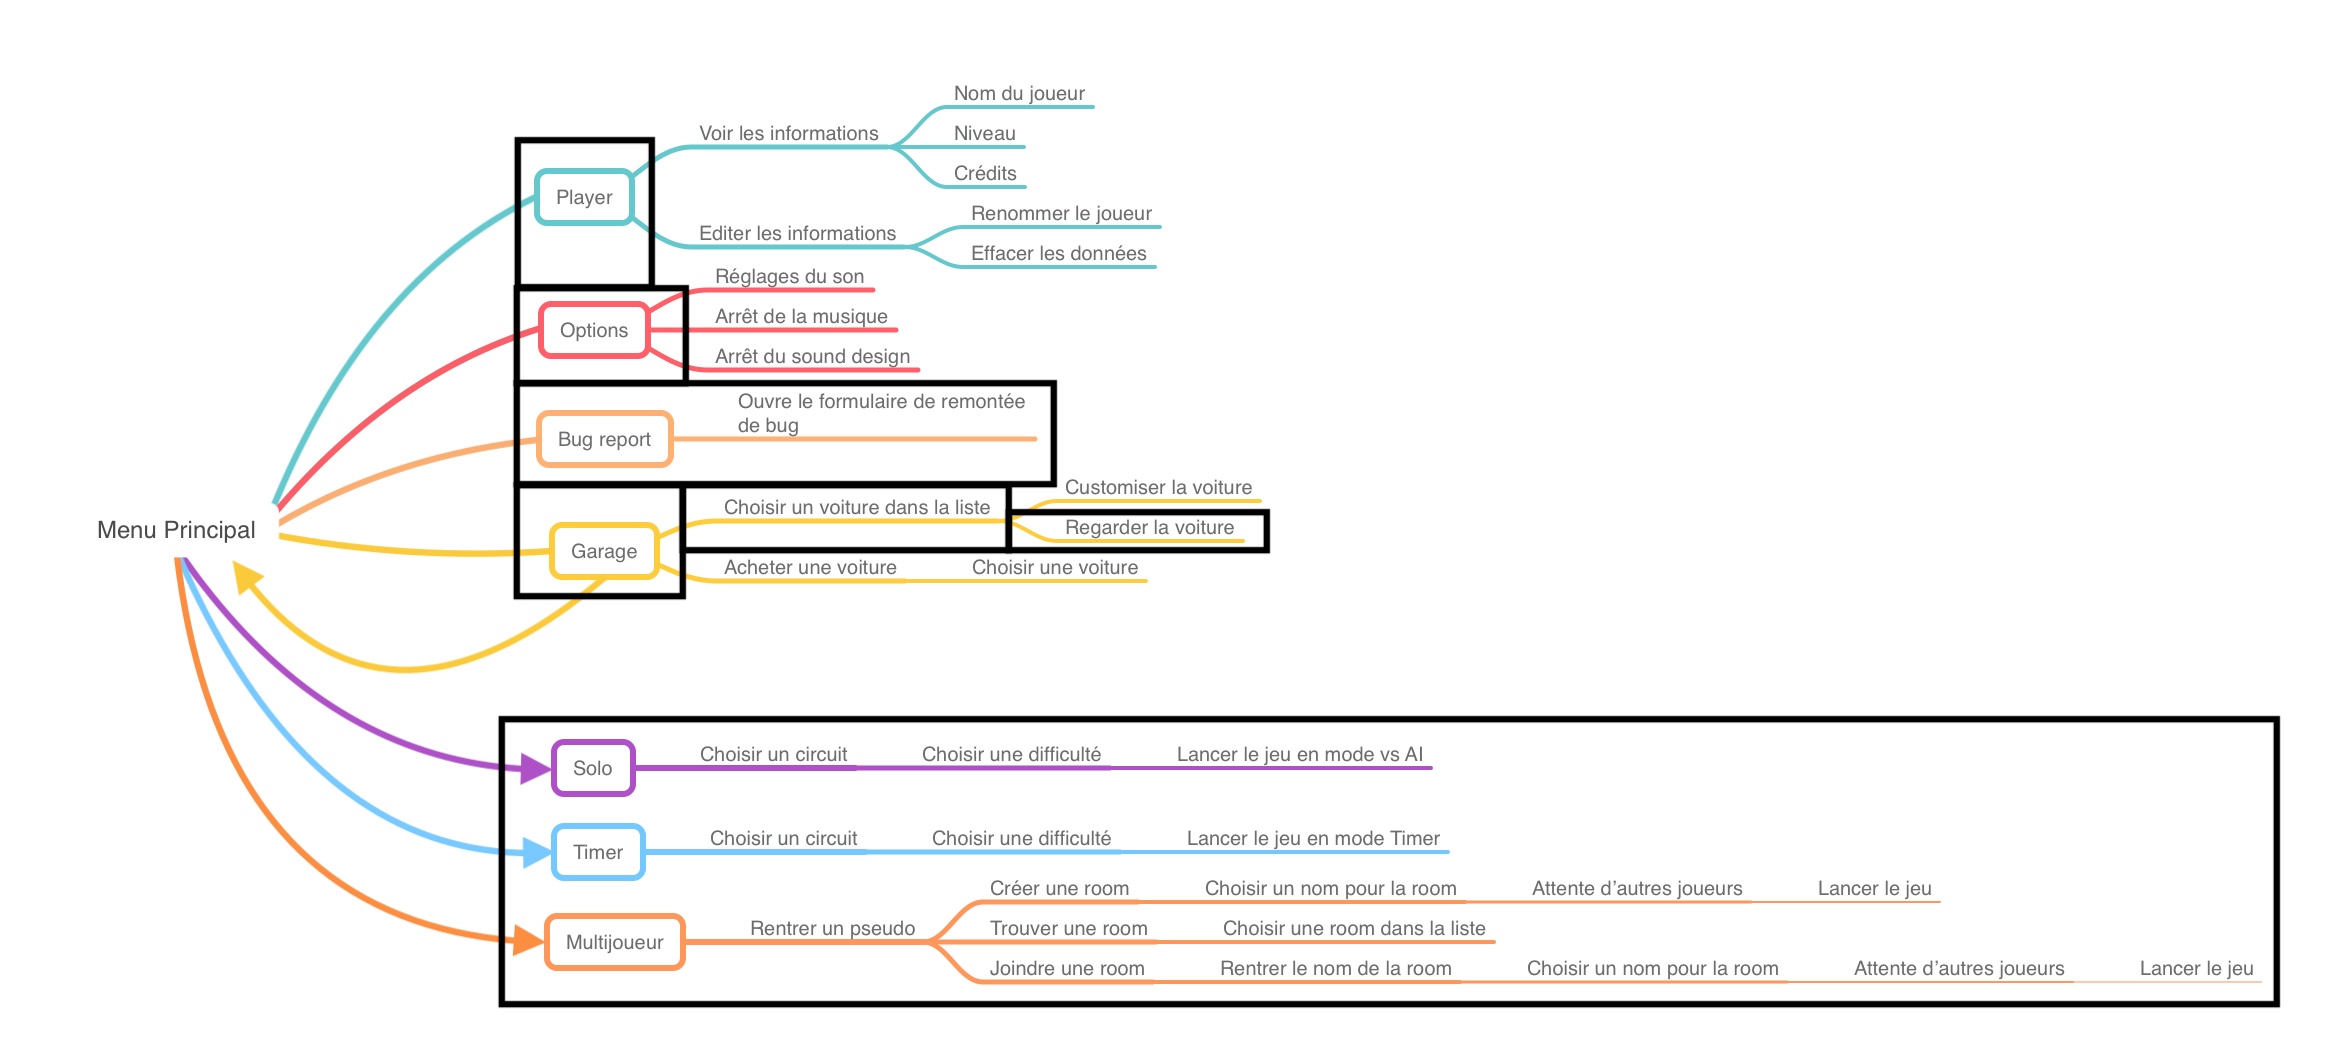
\includegraphics[width=22cm, angle=90]{principalmenu2.png}
            \caption{Arborescence du menu}
            \label{fig:mindmap}
            Ce qui est entouré est déjà implémenté, le reste suivra.
        \end{figure}

        \begin{figure}[h]
            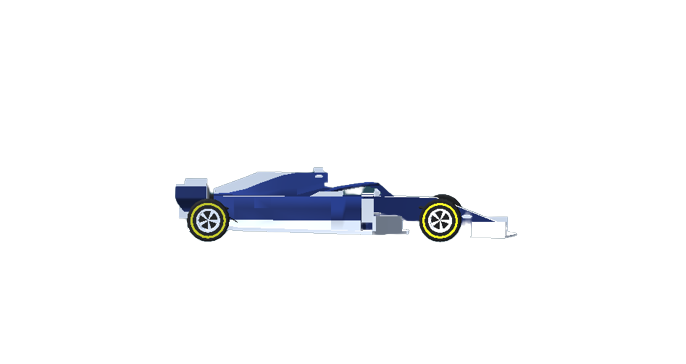
\includegraphics[width=15cm]{f21BG.png}
            \caption{Une Formule 1 créée sur \textsl{Blender}}
            \label{fig:F1}
            \centering
        \end{figure}

        \begin{figure}[t]
            \centering
            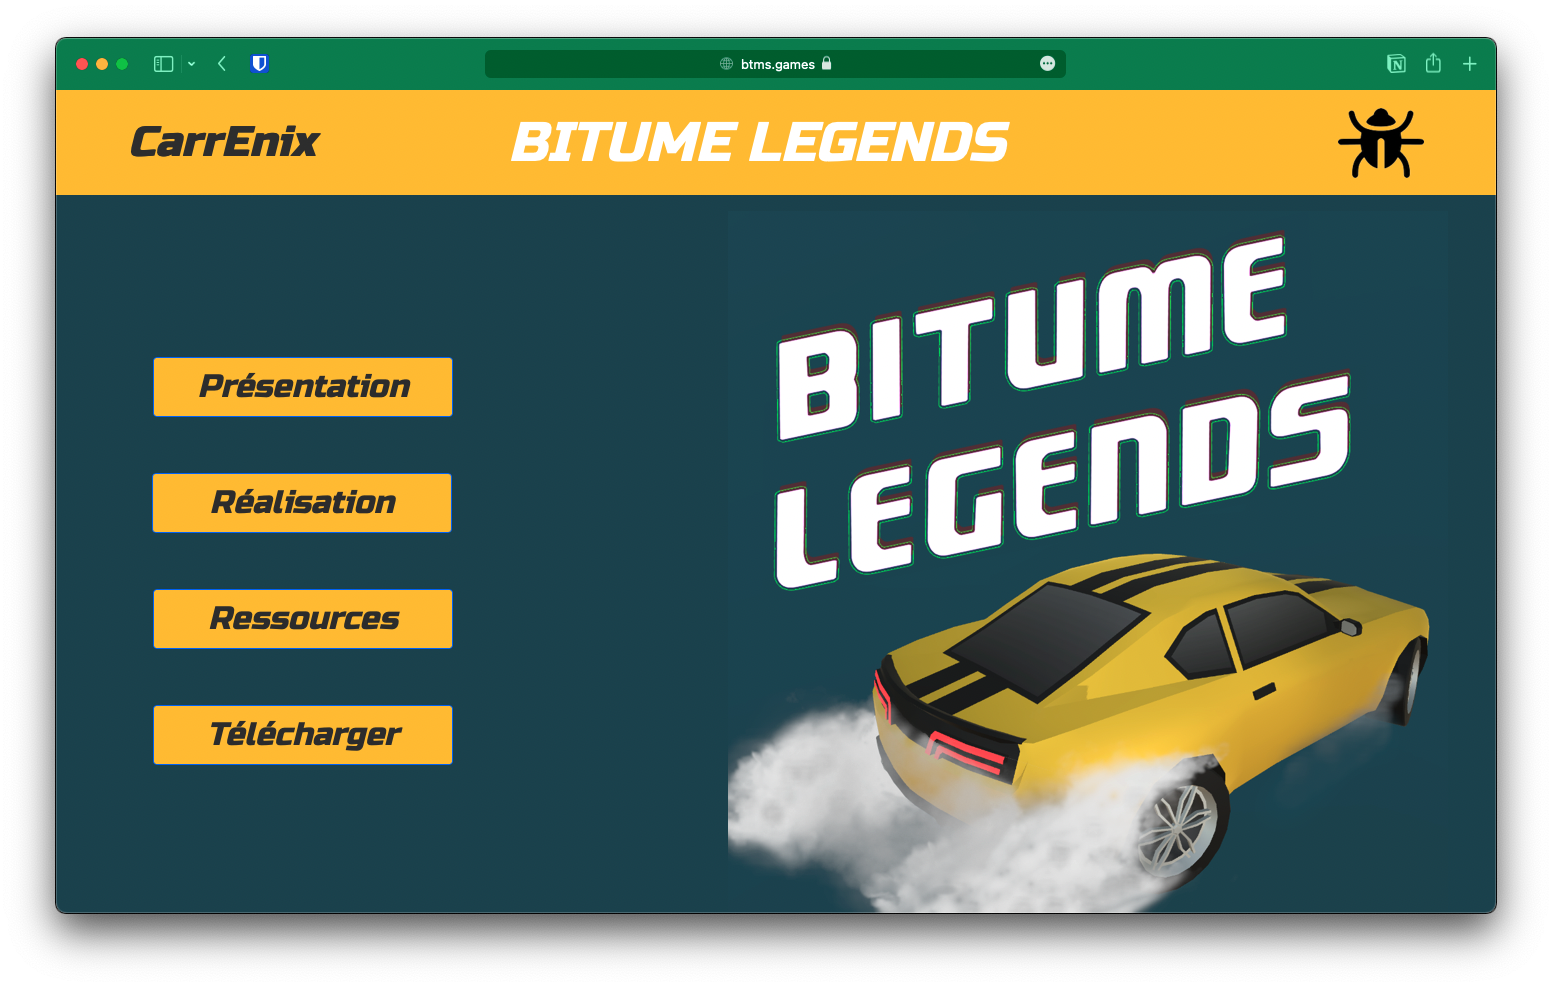
\includegraphics[width=15cm]{site.png}
            \caption{Capture du site Internet}
            \label{fig:site}
            \SITE
        \end{figure}

        \begin{figure}[t]
            \centering
            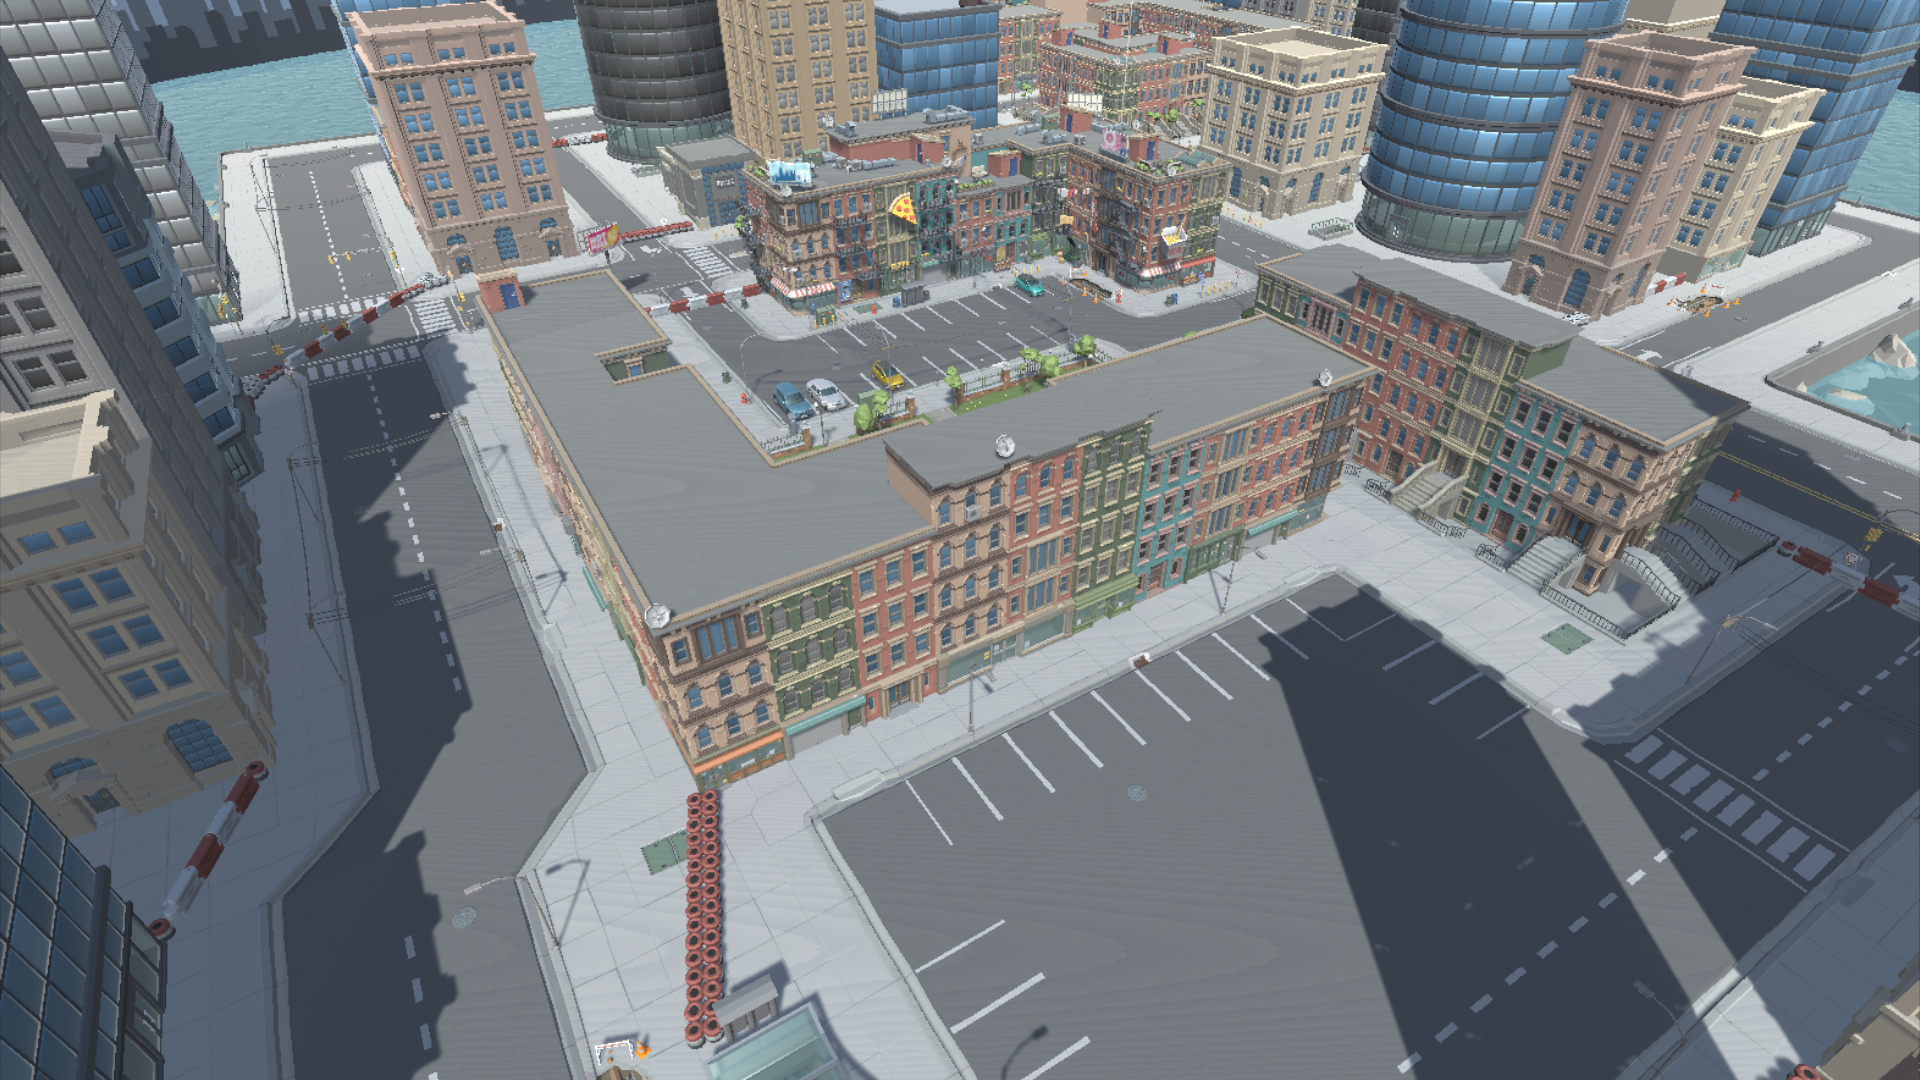
\includegraphics[width=15cm]{trackcity.png}
            \caption{Le premier circuit, \textsl{City}}
            \label{fig:track1}
        \end{figure}

        \begin{figure}[t]
            \centering
            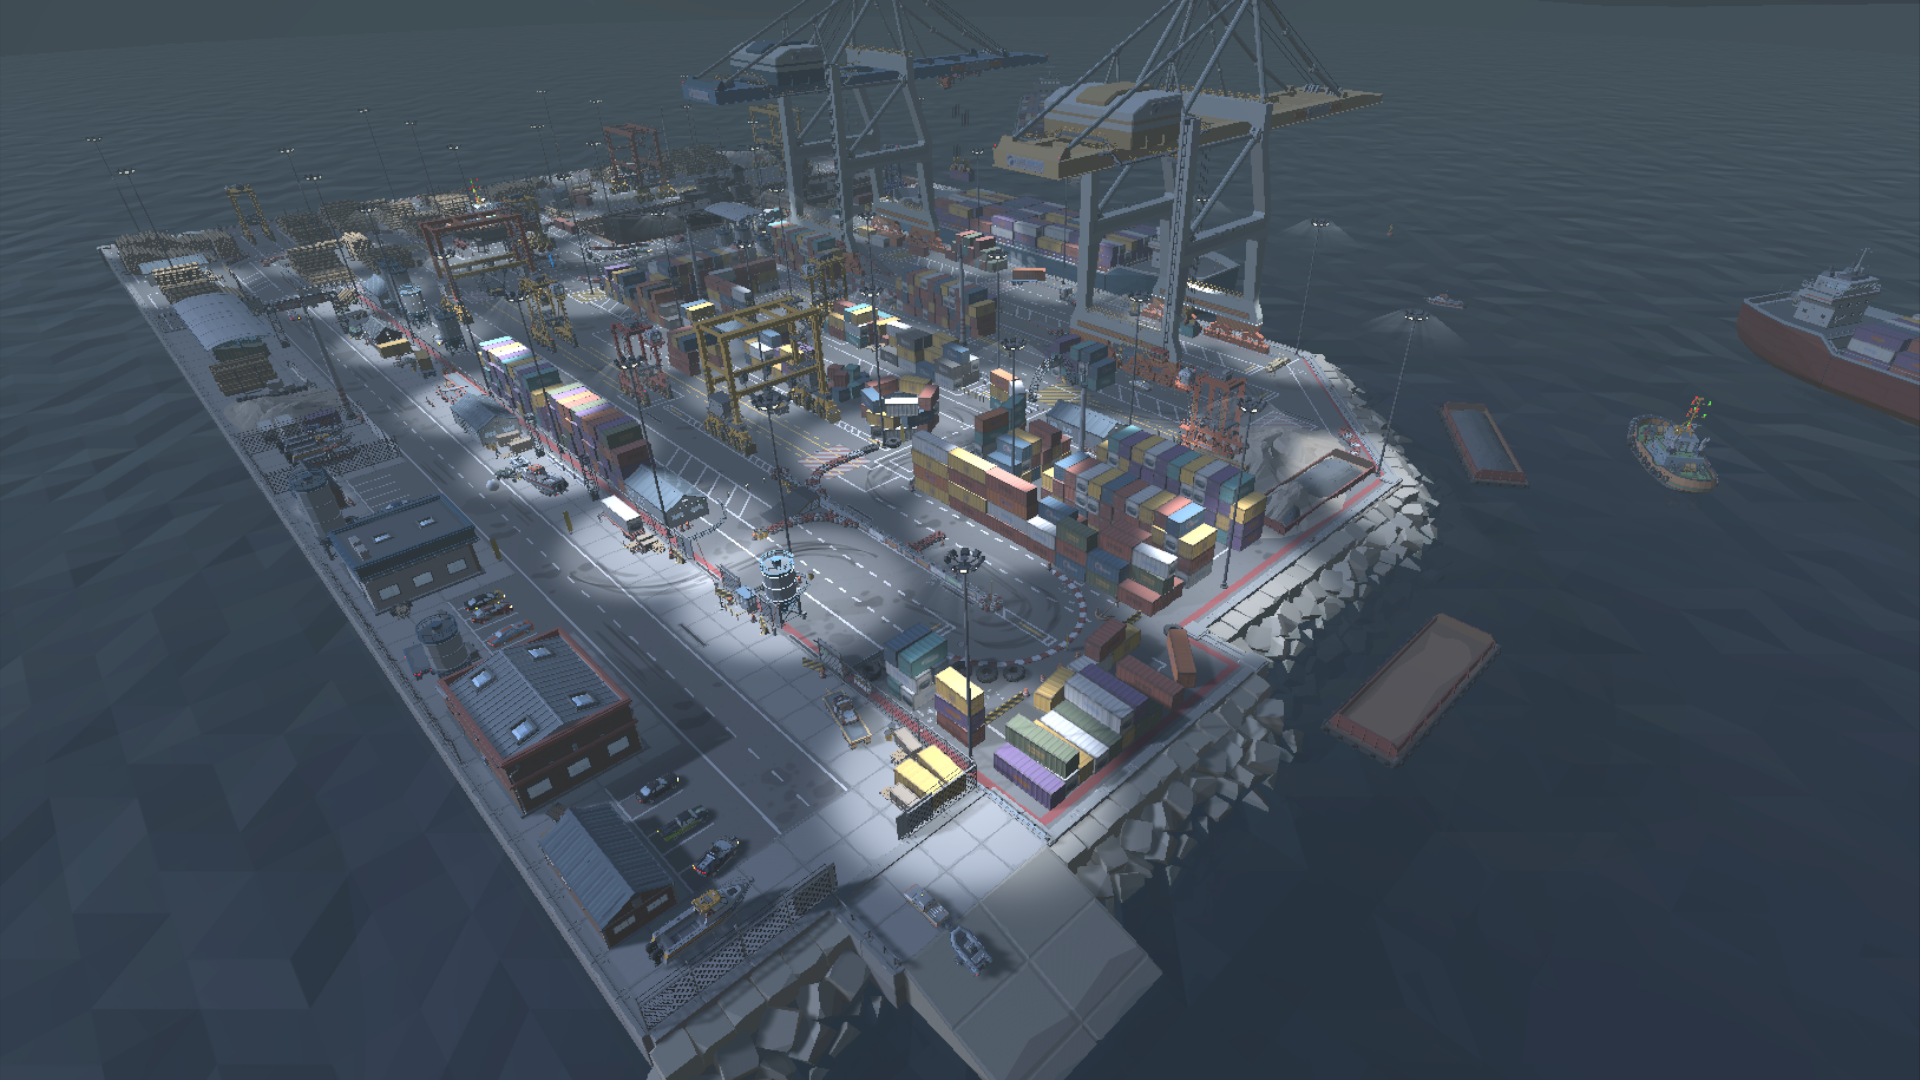
\includegraphics[width=15cm]{trackport.png}
            \caption{Le second circuit, \textsl{Port}}
            \label{fig:track2}
        \end{figure}

\end{document}
